\documentclass{report}
\usepackage{homework}

\usepackage{graphicx}

\solstrue


\definecolor{mygray}{gray}{0.95}
\usepackage{listings}
\lstset{
basicstyle=\small\ttfamily,
columns=flexible,
breaklines=true,
backgroundcolor = \color{mygray},
framexleftmargin = 1em,
xleftmargin = 1em
}

\renewcommand{\hmwkTitle}{Homework 3}

\begin{document}
\mktitle


\begin{problem}

Suppose you have a new computer just set up. \verb|dig| is one of the most useful DNS lookup tool.
You can check out the manual of \verb|dig| at \url{http://linux.die.net/man/1/dig}.
A typical invocation of \verb|dig| looks like:
\verb|dig @server name type|.

Suppose that on April 19, 2017 at 15:35:21, you have issued ``\verb|dig google.com a|'' to get an IPv4 address for \url{google.com} domain from your caching resolver and got the following result:
(If a user just types "dig google.com" the default is type=A)

\begin{lstlisting}

; <<>> DiG 9.8.3-P1 <<>> google.com
;; global options: +cmd
;; Got answer:
;; ->>HEADER<<- opcode: QUERY, status: NOERROR, id: 17779
;; flags: qr rd ra; QUERY: 1, ANSWER: 1, AUTHORITY: 4, ADDITIONAL: 4

;; QUESTION SECTION:
;google.com.			IN	A

;; ANSWER SECTION:
google.com.		239	IN	A	172.217.4.142

;; AUTHORITY SECTION:
google.com.		55414	IN	NS	ns4.google.com.
google.com.		55414	IN	NS	ns2.google.com.
google.com.		55414	IN	NS	ns1.google.com.
google.com.		55414	IN	NS	ns3.google.com.

;; ADDITIONAL SECTION:
ns1.google.com.		145521	IN	A	216.239.32.10
ns2.google.com.		215983	IN	A	216.239.34.10
ns3.google.com.		215983	IN	A	216.239.36.10
ns4.google.com.		215983	IN	A	216.239.38.10

;; Query time: 81 msec
;; SERVER: 128.97.128.1#53(128.97.128.1)
;; WHEN: Wed Apr 19 15:35:21 2017
;; MSG SIZE  rcvd: 180

\end{lstlisting}

\begin{enumerate}

\item What is the discovered IPv4 address of \url{google.com} domain?

\item If you issue the same command 1 minute later, how would ``ANSWER SECTION'' look like?

\item When would be the earliest (absolute) time the caching resolver would contact one of the \url{google.com} name servers again? (for issuing the same  command "dig  google.com a")

\item When would be the earliest (absolute) time the caching resolver would contact one of the \url{.com} name servers? (for issuing the same  command "dig  google.com a")

\end{enumerate}


\begin{answer}{50em}
    Write your answer here

\end{answer}

\end{problem}


% \clearpage
% \begin{problem}

% In most of cases, we rely on caching resolvers to provide recursive DNS query service for us.
% In this task, you will be a human caching resolver using \verb|dig| command as your tool.

% Look up an ``SRV'' resource record (a record that specifies the hostname and port number of a server(s) for some service) for \url{_ndn._udp.ucla.edu.ndn._homehub._autoconf.named-data.net}.

% In your answer, include the exact commands you have used, including IP addresses of the autoritative name servers to which you were sending DNS queries, explain the returned result of each query (what is returned), and indicate for how long you supposed to cache the returned information.

% You can start with one of well-known IP addresses of the DNS root servers, e.g., \url{198.41.0.4}.

% \begin{answer}{30em}
%     Write your answer here

% \end{answer}

% \end{problem}

\clearpage
\begin{problem}

Suppose that you walked into Boelter Hall and get connected to \url{CSD} WiFi network, which automatically gave you IP address of the local caching resolver.
However, initially, it doesn't allow you to do anything unless you type your username and password in a popup window (or if you try to go to any website in your browser).

\begin{enumerate}

\item Explain a mechanism of how does the ``\url{CSD}'' network achieve this / which features of DNS/HTTP make it possible.

\end{enumerate}



\begin{answer}{30em}
    Write your answer here

\end{answer}


\end{problem}


\clearpage
\begin{problem}

  Same context as Problem 2. After you successfully logged in, you can start using the Internet.  Suppose the caching resolver has just rebooted and its cache is completely empty;  RTT between your computer and the caching resolver is $10 ms$ and RTT between the caching resolver and any authoritative name server is $100 ms$; all responses have TTL 12 hours.

\begin{enumerate}
\item If you try to go to \url{ucla.edu}, what would be minimum amount of time you will need to wait before your web browser will be able to initiate connect to the UCLA's web server?

\item What would be the time, if a minute later you will decide to go to \url{ccle.ucla.edu}?

\item What would be the time, if another minute later you will decide to go to \url{piazza.com}?

\item What would be the time, if another minute later you will decide to go to \url{gradescope.com}?

\end{enumerate}

\begin{answer}{24em}
    Write your answer here

\end{answer}

\end{problem}
\clearpage

\begin{problem}
How does SMTP mark the end of a message body? How about HTTP? Can HTTP
use the same method as SMTP to mark the end of a message body? Explain.

\begin{answer}{24em}
    Write your answer here

\end{answer}
\end{problem}

% question 5

\clearpage
\begin{problem}

  Consider the following environment with a local DNS caching resolver and a set of authoritative DNS name servers.
  
  Assume that initially,
\begin{itemize}
    \item the caching resolver cache is empty,
    \item TTL values for all records is 1 hour,
    \item RTT between stub resolvers (hosts A, B, and C) and the caching resolver is 20 ms, 
    \item RTT between the caching resolver and any of the authoritative name servers is 150 ms,
    \item There are no packet losses,
    \item All processing delays are 0 ms
\end{itemize}

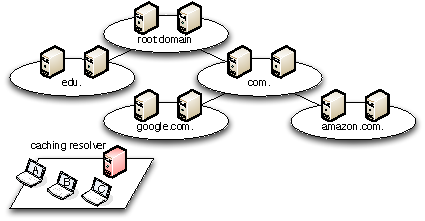
\includegraphics[width=\textwidth]{hw3_problem5.pdf}

\begin{enumerate}
\item At T=0 min, Host-A sends a query for “A record for amazon.com”, and after receiving the answer sends a query for “A record for www.amazon.com”. How long did it take to receive all the answers?

\item At T=40 min, Host-B sends a query for “MX record for google.com” that returns

\begin{lstlisting}

google.com.		3600	IN	MX	10 primary.google.com.
google.com.		3600	IN	MX	30 backup.google.com.
primary.google.com.	3600	IN	A	74.125.28.27
backup.google.com.	3600	IN	A	173.194.211.27

\end{lstlisting}

(Similar to NS records, the DNS server may return “glue” A/AAAA records in addition to the requested MX records.)
How long did it take to get the answer?


\item At T=70 min, Host-C sends a query for “AAAA (IPv6) record for mail.google.com”, following at T=75 mins with a query for “AAAA (IPv6) record for hangout.google.com”. How long did it take for Host-C to receive each of the answers (i.e., relative to T=70min for the first, and relative to T=75 mins for the second)?

\item List DNS records that the caching resolver has at T=90 minutes

% \item At T=100 minutes, all the authoritative servers for .com go offline. Circle the domain names that can be resolved by Host-A? 

% \begin{lstlisting}

% (a) www.google.com    (b) hangout.google.com  (c) doc.google.com
% (d) www.amazon.com    (e) video.amazon.com    (f) aws.amazon.com

% \end{lstlisting}

\end{enumerate}

\begin{answer}{24em}
    Write your answer here

\end{answer}

\end{problem}

\end{document}
